%!TeX program = xelatex
\documentclass[12pt,hyperref,a4paper,UTF8]{ctexart}
\usepackage{USTCReport}

%%-------------------------------正文开始---------------------------%%
\begin{document}

%%-----------------------封面--------------------%%
\cover

%%------------------摘要-------------%%
\newpage
\begin{abstract}

2021年美国国家点火装置（NIF）首次实现聚变增益（$Q>1$），为激光惯性约束聚变能源（IFE）领域带来了里程碑式突破。本研究基于Scopus数据库构建包含243篇核心文献的三层引文网络，采用Wu与Yan提出的独奏引用（Solo Citations, SC）指标体系，系统分析IFE领域的知识扩散模式与学术引用结构，评估NIF点火是否引发了实质性的科学范式转型。结果表明：IFE领域独奏引用占比自1992年以来整体波动下降，呈现渐进式发展特征而非革命性跃迁；知识产出高度集中于美、中、法三国，体现该领域典型的大科学特征。本研究验证了$R_{\mathrm{SC}}$指标在颠覆性创新评估中的有效性，为聚变能源战略决策提供科学计量学视角的实证参考。

\vspace{1cm}

\textbf{关键词：}惯性约束聚变；独奏式应用；科学计量学；

\end{abstract}

\thispagestyle{empty} % 首页不显示页码

%%--------------------------目录页------------------------%%
\newpage
\tableofcontents

%%------------------------正文页从这里开始-------------------%
\newpage

%%可选择这里也放一个标题
%\begin{center}
%    \title{ \Huge \textbf{{标题}}}
%\end{center}

\section{引言}
2021年美国国家点火装置（NIF）首次实现靶丸聚变产额大于激光输入能量\cite{abu2022lawson}，标志着激光惯性约束聚变能源从基础研究向能量可行性迈出了里程碑式的一步。
这一突破使得惯性约束聚变能源（Inertial Confinement Fusion Energy, IFE），尤其是激光间接驱动路径，被视为未来清洁能源的。

然而，一项技术或领域是否真正“颠覆”现有知识体系，不仅取决于其物理指标的跃升，更体现在它对后续研究的知识扩散模式与学术引用结构上。传统的文献计量方法多聚焦于影响力或热度，难以刻画“根本性重构”的效应。近年来，引文特征分析为识别颠覆性创新提供了新的工具。
若NIF点火确实引发了IFE领域的范式转型，那么其核心成果的引用模式应呈现出高原创性和对经典理论的替代性引用等特征。
因此，本研究拟聚焦于NIF点火里程碑论文及其后续关键文献的引用网络，通过独奏式引用指标\cite{wu2019solo}，判断激光惯性约束聚变能源领域是否发生了实质性的科学变革，以期为颠覆性成果的早期识别方法提供实证依据，同时为聚变能源战略决策提供参考。

\section{实验内容}
    \subsection{数据采集}
    本研究的数据源自爱思唯尔（Elsevier）Scopus数据库，通过其官方应用程序编程接口（API）进行自动化采集。
        
        \subsubsection{构建检索策略}
        激光惯性约束聚变领域发展历史较长，从1950年代开始，其用词变化较大，本次实验检索时采用的检索表达式为: 
            
            \begin{equation}
                \text{TITLE-ABS-KEY ( "laser" AND " inertial confinement fusion" AND "energy" )}
                \label{检索式}
            \end{equation}

        \autoref{检索式}可以保证检索到的文献主要关注激光惯性约束聚变领域，避免了大量磁约束聚变等其他相关领域的文献的干扰的同时，更多地聚焦于能源应用方向。

        将检索到的文献经筛选后以 CSV 文件形式导出，包含文献的标题、作者、DOI、发表年份、引用次数等信息，方便后续大批量引文数据的采集和处理。

        \subsubsection{批量采集}
        本研究使用 pybliometrics —— 一个开源的 Python 接口库，通过 Scopus 官方 API 批量获取文献的引用关系数据，
        pybliometrics 封装了 Scopus API 的多种访问端点，提供统一的接口类进行数据检索、缓存和管理，相比直接调用原始 API 能显著降低开发复杂度并提升采集效率。
        通过多个 API keys 轮询和线程并行采集，本研究能够快速获取文献的引用关系数据，确保研究的效率和准确性。

    \subsection{元数据处理}

        \subsubsection{元数据}
        在科学计量学研究中，文献元数据（metadata）是指描述学术出版物基本属性的结构化数据集合，包括标题、作者、发表年份、机构、国家或地区、关键词、被引次数等\cite{singh2024exploring}。
        这些元数据字段为量化分析提供了基础维度，使得文献集合可以按时间、地域、主题等类别被划分与统计。
        
        \subsubsection{元数据字段}
        本研究从Scopus导出的CSV数据中提取以下关键元数据字段：
        \begin{enumerate}
            \item \textbf{发表年份}（Year），用于按时间轴对文献进行分组、追踪领域演进趋势，并在年度层面计算SC占比的均值与极值；
            \item \textbf{国家或地区}（Country），标识作者所属机构所在的地理区域，可用于分析各国在IFE领域的研究投入差异与知识产出格局；
            \item \textbf{文献标题}（Title）与\textbf{关键词}（Keywords），辅助判断文献的主题相关性；
            \item \textbf{总被引次数}（Cited by），作为SC占比计算公式中的分母，反映文献的整体学术影响力。上述元数据字段与引文网络数据相互补充，共同构成了完整的分析数据集。
        \end{enumerate}

    \subsection{引文数据处理}

        \subsubsection{引文网络构建}

        经前述批量采集步骤，对采集到的3138文献进行再筛选保留引用次数较高的论文，同时剔除一些数据库引用关系不全的文献数据。
        覆盖了243篇被引次数在50次以上的论文，揭示激光惯性约束聚变领域的核心研究内容的同时，也忽略了低引用次数论文可能带来的噪声。
        
        每条目标文献均获得三类结构化数据：（1）其参考文献列表；（2）其施引文献列表；（3）各施引文献的参考文献列表。本研究以此为每篇目标文献构建一个以该文献为核心的三层引用单向网络，网络节点包括目标文献自身、其参考文献集合、其施引文献集合以及施引文献的参考文献集合。

        \subsubsection{独奏式引用指标的计算}

        本研究采用Wu与Yan提出的独奏式引用（Solo Citations, SC）指标体系来度量学术论文的颠覆性\cite{wu2019solo}。该体系将施引文献对目标文献的引用行为划分为三类：    

        \begin{itemize}
            \item \textbf{独奏式引用（SC）}：施引文献仅引用目标文献，而未引用目标文献的任何一篇参考文献。此类引用表明目标文献已在知识传播中脱离其原始文献背景、形成了独立的影响力。
            \item \textbf{二重引用（DC）}：施引文献同时引用目标文献及其至少一篇参考文献。此类引用表明目标文献与其参考文献在后续研究中被作为整体知识体系共同采纳。
            \item \textbf{序曲引用（PC）}：施引文献仅引用目标文献的参考文献而未引用目标文献本身。此类引用表明该文献的知识溯源仍可追溯至更早期的知识基础。
            \item 其中，$DC+PC$的数量为一篇文献的总被引次数。
        \end{itemize}

        若一篇论文具有颠覆性，则后继研究者在引用该论文时，将更倾向于绕过其参考文献而直接引用该论文本身。因此，$R_{\mathrm{SC}}$值越高，表明该论文对既有知识体系的替代性越强，其颠覆性潜力越大。Wu与Yan进一步指出，在多种候选指标中，$SC$、$SC-DC$、$SC/(SC+DC)$以及$(SC-DC)/(SC+DC)$四项指标在逻辑与实证层面均具有合理性。本次实验中，采用$R_{\mathrm{SC}}=SC/(SC+DC)$作为评估指标。

        在本项目中，先定义为二值属性SC：对于目标文献$\text{F}$的每一篇施引文献$\text{C}$，若$\text{C}$引用了$\text{F}$但未引用$\text{F}$的任何参考文献，则$\text{C}$被标记为$\text{F}$的一篇独奏式引用，SC赋值为1；否则SC赋值为0。每篇目标文献的SC总量即为其所有施引文献中SC=1的数量之和。

        \subsubsection{数据处理流程}

        完整的数据处理流水线包含四个阶段：

            \textbf{阶段一：基础数据采集。}基于Scopus导出的文献EID列表，在Python环境中调用pybliometrics库的AbstractRetrieval和ScopusSearch接口，逐篇获取参考文献列表与施引文献列表。该阶段记录每篇目标文献的参考文献列表和施引文献列表，建立一级引用关系。

            \textbf{阶段二：二级引用关系展开。}使用多进程并行和API轮询机制高效遍历阶段一获取的每篇施引文献，再次调用AbstractRetrieval接口获取每篇施引文献的参考文献列表。该阶段为每篇目标文献建立了由施引文献到参考文献的映射关系。

            \textbf{阶段三：引文网络构建与SC计算。}设计EIDNetworkBuilder类，遍历网络中所有目标文献的三级结构，利用阶段一和阶段二的数据构建三层引文有向边网络。对每个目标文献节点，依据前述SC判定规则进行二值标注，并将结果输出为含SC标记节点的列表文件。

            \textbf{阶段四：指标聚合与统计。}设计ProcessEID函数，基于Python实现，批量读取Scopus原始导出数据中的年份与总被引次数（Cited by），结合各文献的SC总量，计算每篇文献的独奏式引用占比：

        \begin{equation}
            R_{\mathrm{SC}} = \frac{\mathrm{SC}_{\mathrm{tot}}}{\mathrm{SC+DC}}
            \label{SCratio}
        \end{equation}

        \autoref{SCratio}中$\mathrm{SC_{tot}}$为该文献的独奏式引用总数，$\mathrm{Cit}$为该文献的总被引次数。该比值反映了文献的引用中独立于其知识背景的比例。
        对所有文献按年份分组后，计算各年份发表文献的$R_{\mathrm{SC}}$均值、最大值与最小值，生成数据汇总表格，供后续统计分析与可视化使用。

        % \subsubsection{激光惯性约束聚变领域的特殊性}

        % 在激光惯性约束聚变（IFE）领域，知识的继承性极强。从1960年代激光器发明至今，该领域经历了从直接驱动到间接驱动、从氘氚燃料到双壳层靶丸等多个范式演进阶段。2021年美国国家点火装置（NIF）首次实现靶丸聚变产额大于激光输入能量（$Q>1$），被广泛视为惯性约束聚变从基础物理验证迈向聚变能源可行性的转折点。

        % 在此背景下，若NIF点火确实引发了领域的范式转型，则应可观测到以下引文特征变化：点火相关核心论文的SC值在2021年后应呈现显著上升趋势，表明后续研究者更倾向于直接引用点火成果本身，而不再依赖其早期的理论参考文献。反之，若SC值在年度间波动不大，则说明该领域的知识积累呈渐进式发展而非革命性跃迁。

        % 此外，IFE领域具有典型的“大科学”特征——每项突破性成果通常建立在大型激光装置的实验数据之上，其引文网络呈现高度的设备依赖性。因此，SC指标在IFE领域的适用性分析还需考虑装置更替带来的引文结构自然变化，以避免将硬件迭代误判为科学颠覆。



\section{实验结果}

    \subsection{基于元数据的指标统计}
    根据检索到的3138篇文献元数据绘制的\autoref{metadata1}显示，领域年均发文量在1980年代激光惯性聚变能源概念提出至今，呈现波动上升趋势。
    而\autoref{metadata2}显示，作者国籍分布主要集中在美国、中国、法国等国家，集中度较高。
    这可能是因为激光惯性约束聚变领域的研究高度依赖大型激光装置如NIF、神光系列、LMJ，且与国家利益密切相关。

    \begin{figure}[!htbp]
        \centering
        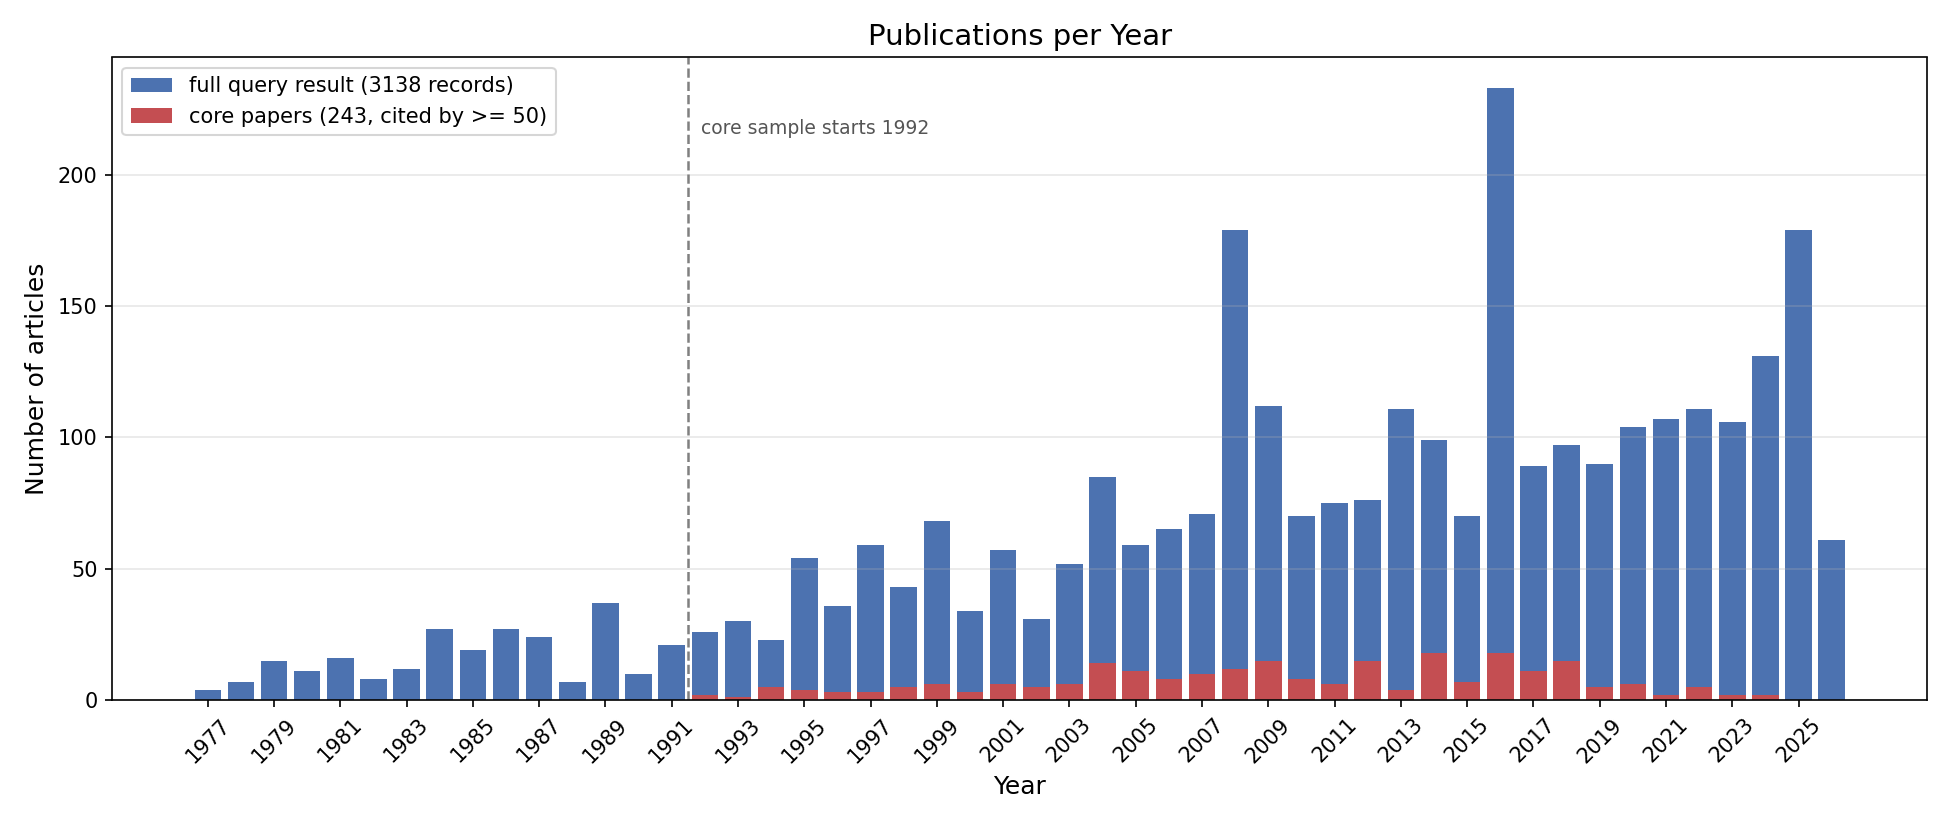
\includegraphics[width =.8\textwidth]{figures/article_year.png}
        \caption{年均发文量随年份变化趋势}
        \label{metadata1}
    \end{figure}

    \begin{figure}[!htbp]
        \centering
        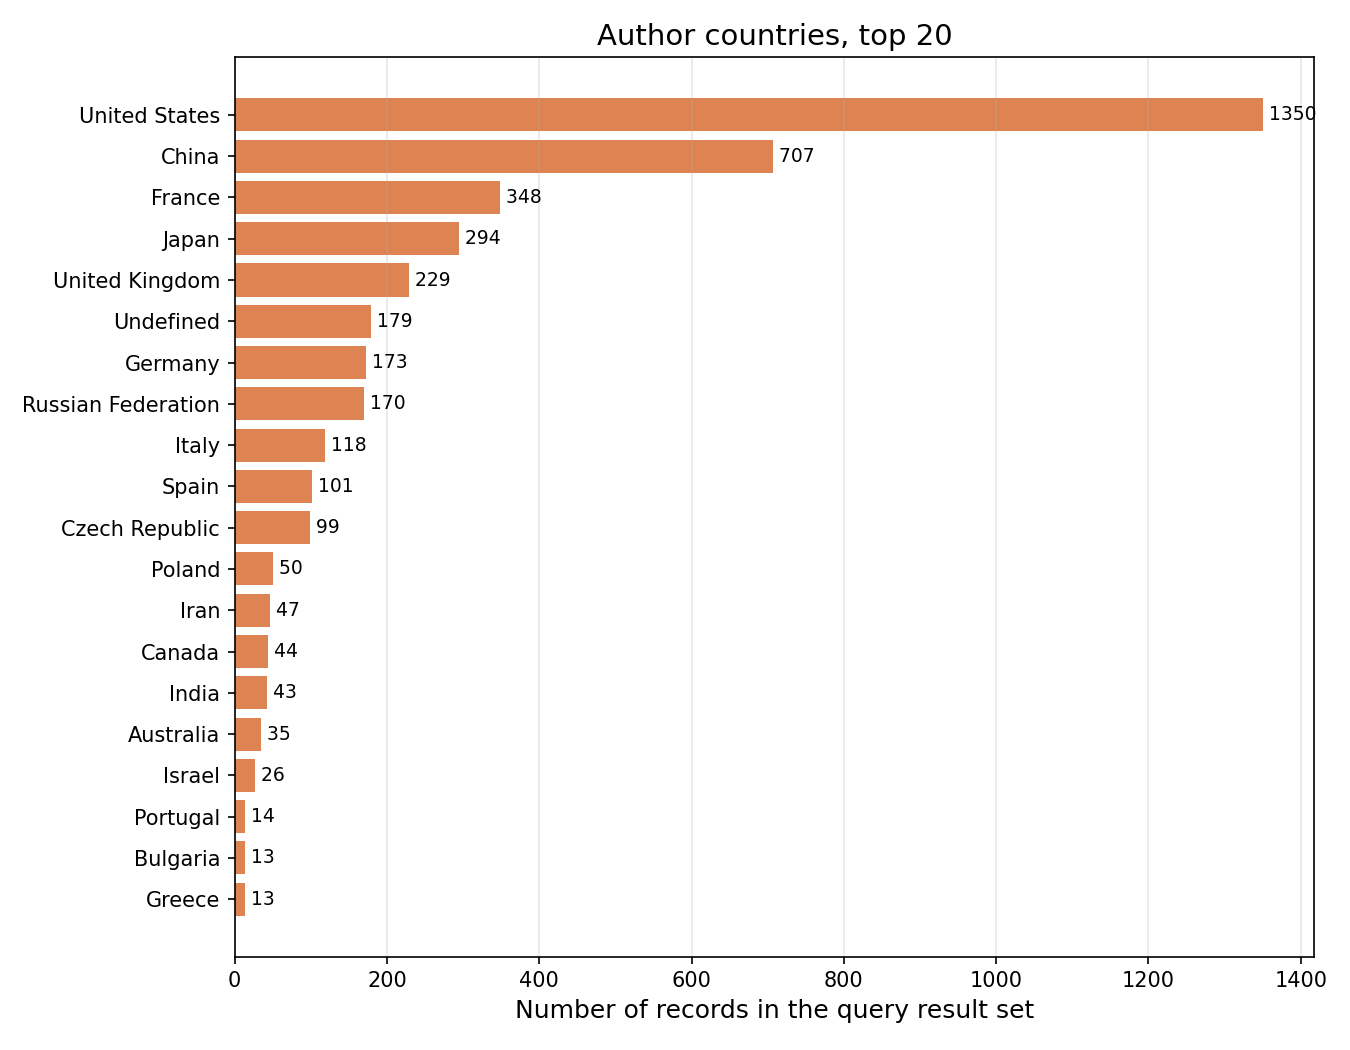
\includegraphics[width =.8\textwidth]{figures/author_nation.png}
        \caption{作者国籍分布}
        \label{metadata2}
    \end{figure}


    \subsection{基于引文网络的指标统计}

    \subsubsection{总体概览}
        根据引文引文网络，对文献的独奏式引用占比按年份分组后，计算各年份$R_{\mathrm{SC}}$的均值、最大值与最小值，绘制\autoref{yearly_rate}发现：
        \begin{figure}[!htbp]
            \centering
            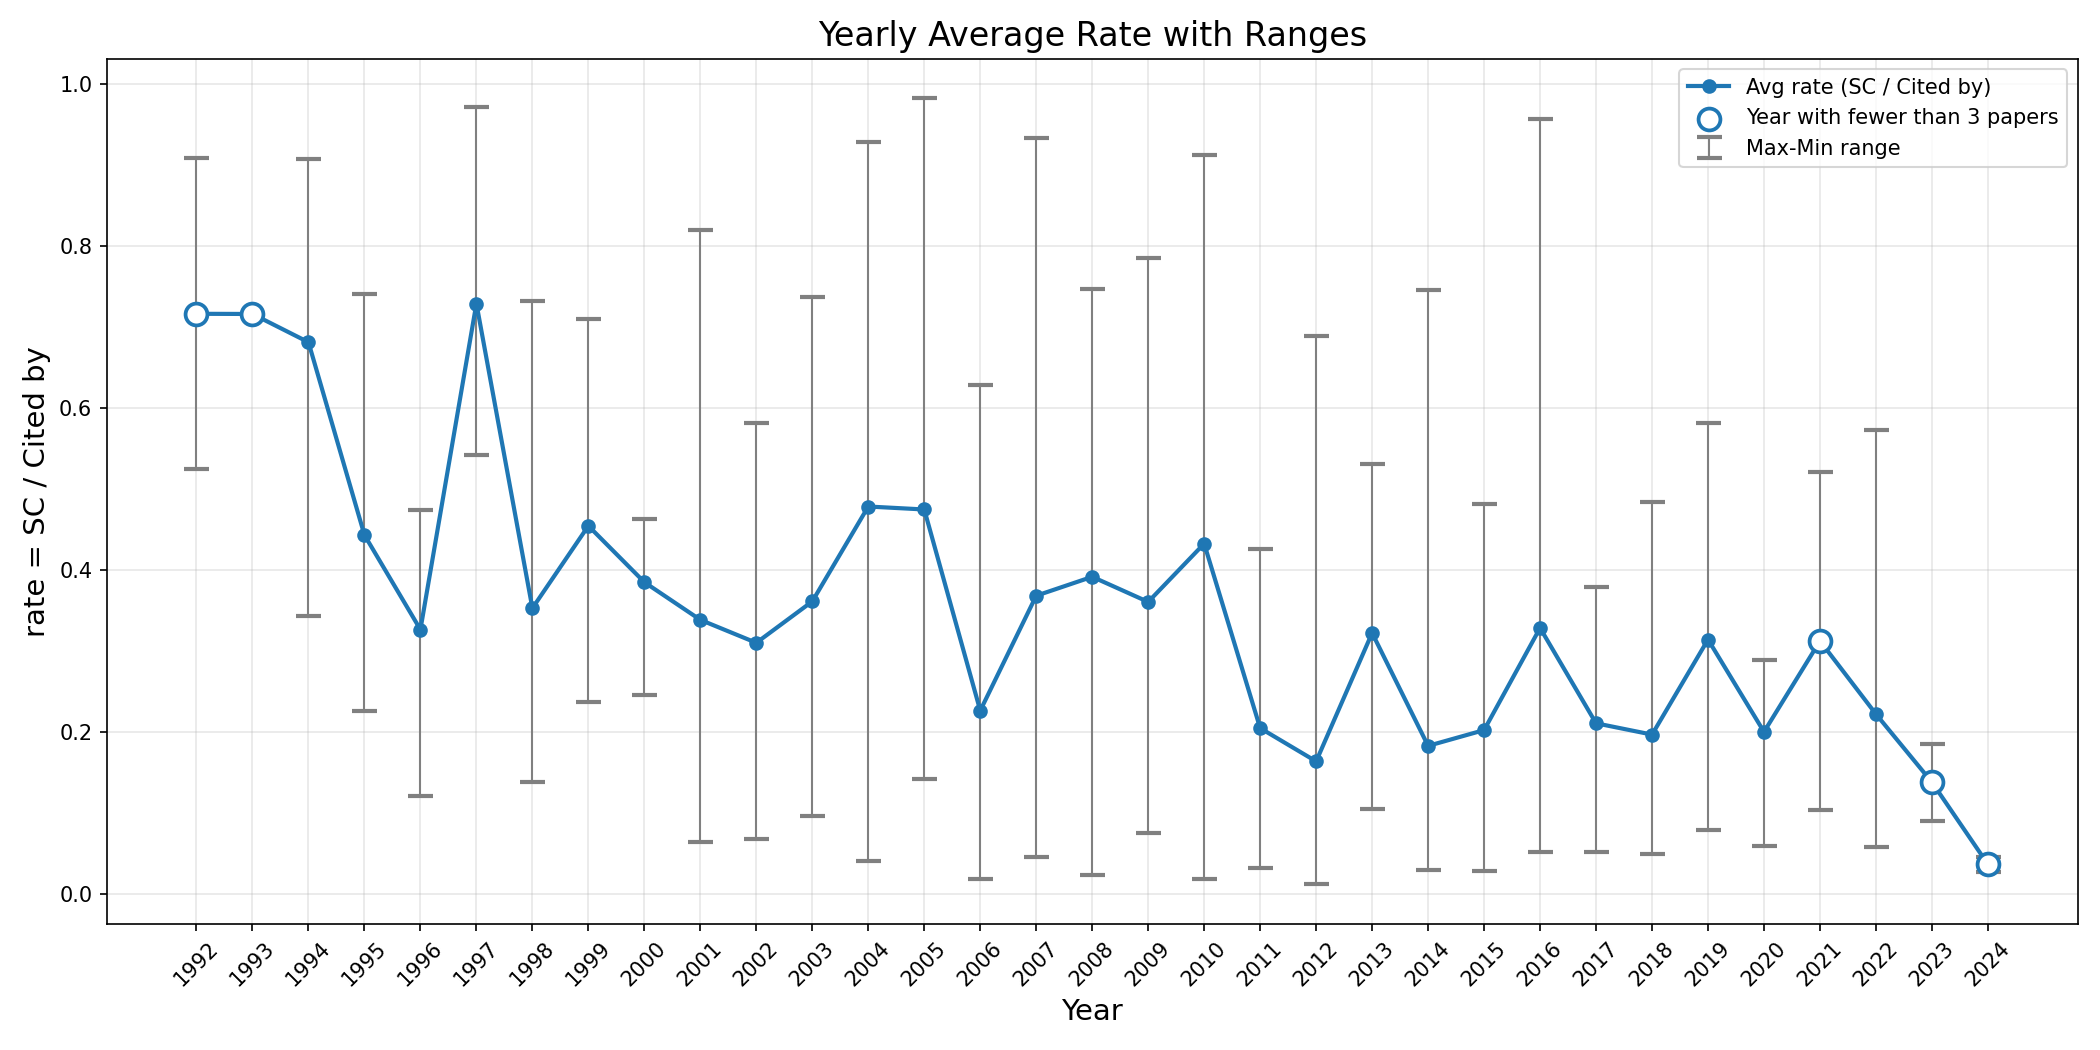
\includegraphics[width =.8\textwidth]{figures/washed_yearly_rate.png}
            \caption{独奏式引用占比随年份变化趋势}
            \label{yearly_rate}
        \end{figure}
        激光惯性约束聚变领域中，独奏式引用占比在1992年后整体波动下降，可以推测该领域的知识积累呈渐进式发展而非革命性跃迁，惯性约束聚变领域持续稳步发展。

        这与2013年美国National Research Concil在NIF没有完成阶段目标时对惯性聚变能源的前景评估\cite{nrc2013assessment}印证，惯性约束聚变能源科技发展过程虽可能遭遇挫折，阶段目标的实现迟于计划，但总体目标仍然有望实现。

    \subsubsection{对点火本身的分析}
        NIF实现点火的原始文献\cite{abu2022lawson}不在样本中。其被引SC占比为 $79/475\approx 0.1663$ 小于样本SC占比的当年均值0.2224，可以说明该项成果的延续性强于颠覆性，表明NIF点火是之前研究范式的延续和重要里程碑。
        


\section{实验结论}

    本研究以激光惯性约束聚变能源（IFE）领域为对象，基于Scopus数据库构建了包含243篇核心文献的三层引文网络，采用Wu与Yan提出的独奏式引用（Solo Citations, SC）指标体系，系统分析了该领域的知识扩散模式与学术引用结构，进而评估2021年美国国家点火装置（NIF）首次实现$Q>1$这一里程碑事件是否引发了实质性的科学范式转型。主要结论如下：

    \textbf{（1）激光惯性约束聚变领域的知识积累呈现渐进式发展特征。}基于引文网络的独奏式引用占比$R_{\mathrm{SC}}$分析表明，该指标在1992年后整体波动下降，而非在2021年NIF点火前后出现显著跃升。这说明NIF点火成果在引文结构上仍然嵌于既有知识体系之中，后续研究者倾向于同时引用点火成果及其参考文献，形成"二重引用"而非"独奏式引用"。因此，NIF点火应被视为已有范式的延续与重要里程碑，而非完全的路径创新。

    \textbf{（2）IFE领域具有典型的"大科学"特征，知识生产呈现高度的地缘特征。}基于元数据的发文量与作者国籍分布分析显示，自1980年代激光聚变能源提出至今，领域年均发文量呈波动上升趋势；同时，知识产出高度集中于美国、中国、法国等国家。这种集中性与IFE领域对大型激光装置（如NIF、神光系列、LMJ）的强依赖性一致，也反映了聚变能源研究对国家长期战略投入的深刻依赖。

    \textbf{（3）独奏式引用指标为评估颠覆性创新提供了有效的实证工具。}本研究验证了$R_{\mathrm{SC}}$指标在IFE领域的适用性：当领域的SC占比呈现持续下降趋势时，表明该领域的知识演进模式为渐进式积累；为$R_{\mathrm{SC}}$指标在更多领域的应用提供参考。

    综上所述，2021年NIF点火虽然在工程实践意义上实现了聚变增益的历史性突破，但从科学计量学的引文结构视角来看，该事件尚未引发IFE领域知识体系的根本性重构。未来该领域的突破性潜力，可能取决于后续的经济效益讨论和能量利用途径等角度能否取得进一步的颠覆性进展。



\section{讨论}
    \subsection{验证$R_{\mathrm{SC}}$指标的适用性}
    在清洗后的数据中选择了张杰提出双锥点火方案的文献\cite{zhang2020doublecone}和Hurricane O.A.回顾美国惯性约束聚变实验的文献\cite{hurricane2023physics}为具体案例。
    
    前者为理论创新$R_{\mathrm{SC}}\approx0.2886$，后者为实验综述$R_{\mathrm{SC}}\approx0.1858$，可以证明在IFE领域中，该指标具有一定的区分度和应用价值。



    \subsection{局限性}
    本实验存在的局限性有；
    \begin{itemize}
        \item 文献数据规模较小，没有验证结论稳定性和关键变量敏感性。
        \item 三层引用网络关系展开需求数据过多，计算资源消耗效率低。
        \item 仅考虑了文献的独奏式引用占比，未考虑其他的引用指标。没有具体讨论引用习惯、预印本文献影响等情形时，该指标仍具有一定局限性。
        \item 未与数据库平均基准或相似邻域进行对比，无法判断各类现象和指标的强度。
    \end{itemize}

    \subsection{未来展望}
    未来研究可以考虑从以下几个方面展开：
    \begin{itemize}
        \item \textbf{增加数据采集范围，覆盖更多核心文献。}通过优化算法和本地数据库构建，可以实现更大规模的引文网络构建，提升分析的代表性和结论的稳健性。
        \item \textbf{考虑其他引用指标。}探索各类文献计量指标在IFE领域的适用性，构建多维度的颠覆性评估体系。
        \item \textbf{与数据库平均基准或相似邻域进行对比。}研究该指标在不同领域不同时间段的表现，判断IFE领域的独奏式引用占比规律是否具有独特性和显著性。
    \end{itemize}





















































% \section{模板说明}
% 本模板主要适用于一些课程的平时论文以及期末论文，默认页边距为2.5cm，中文宋体，英文Times New Roman，字号为12pt（小四）。

% 编译方式：\verb|xelatex -> bibtex -> xelatex*2|


% 默认模板文件由以下四部分组成：
% \begin{itemize}
%     \item \texttt{main.tex} 主文件
%     \item \texttt{reference.bib} 参考文献，使用bibtex
%     \item \texttt{USTCReport.sty} 文档格式控制，包括一些基础的设置，如页眉、标题、姓名等
%     \item \texttt{figures} 放置图片的文件夹
% \end{itemize}

% 第一次使用时需前往\texttt{USTCReport.sty} 对标题、姓名、学号、院所、页眉等进行设置，设置完后即可一劳永逸，封面logo亦可替换

% 默认带有封面页以及目录页，页码从目录页开始

% \section{一些插入功能}
% \subsection{插入公式}
% 行内公式$v-\varepsilon+\phi=2$。

% 插入行间公式如\autoref{Euler}：
% \begin{equation}
%     v-\varepsilon+\phi=2
%     \label{Euler}
% \end{equation}

% \subsection{插入图片}
% USTC校徽如\autoref{USTC}所示，注意这里使用了\verb|~\autoref{}|命令，也就是会自动生成“图”“式”等前缀，无需手动输入。

% \begin{figure}[!htbp]
%     \centering
%     
\includegraphics[width =.4\textwidth]{figures/ustc_logo_side.pdf}
%     \caption{中国科学技术大学}
%     \label{USTC}
% \end{figure}

% 插入上面图片的代码：

% \begin{verbatim}
%     \begin{figure}[!htbp]
%         \centering
%         \includegraphics[width =.4\textwidth]{figures/USTC_logo.pdf}
%         \caption{中国科学技术大学}
%         \label{USTC}
%     \end{figure}
% \end{verbatim}

% \subsection{插入文本框}
% 本模板定义了一个圆角灰底的文本框，使用简化命令\verb|\tbox{}|即可，如果你不喜欢，可以前往 \texttt{USTCReport.sty}对其进行修改。

% \tbox{
%     这是一个圆角灰底的文本框
% }

% \subsection{插入表格}
% 本模板文件如\autoref{doc}所示。
% \begin{table}[!htbp]
%     \centering
%     \begin{tabular}{l  | l}
%         \hline
%         文件名                  & 说明         \\
%         \hline
%         \texttt{main.tex}       & 主文件       \\
%         \texttt{reference.bib}  & 参考文献     \\
%         \texttt{USTCReport.sty} & 文档格式控制 \\
%         \texttt{figures}        & 图片文件夹   \\
%         \hline
%     \end{tabular}
%     \caption{本模板文件组成}
%     \label{doc}
% \end{table}

% %\section{定理环境}
% %\begin{Theorem}
% %\end{Theorem}
% %
% %\begin{Lemma}
% %\end{Lemma}
% %
% %\begin{Corollary}
% %\end{Corollary}
% %
% %\begin{Proposition}
% %\end{Proposition}
% %
% %\begin{Definition}
% %\end{Definition}
% %
% %\begin{Example}
% %\end{Example}
% %
% %\begin{proof}
% %\end{proof}

% \subsection{插入参考文献}
% 直接使用\verb|\cite{}|即可。

% 例如：


% \textit{ 此处引用了文献\cite{0Isaac}。此处引用了文献\cite{2016The}}


% 引用过的文献会自动出现在参考文献中。

% \section{写在最后}
% \subsection{发布地址}
% \begin{itemize}
%     \item Github: \url{https://github.com/jweihe/USTC_Latex_Template}
%     \item Overleaf:  \url{https://www.overleaf.com/latex/templates/USTCke-cheng-lun-wen-mo-ban/bcwvxncqffkw}
% \end{itemize}














%%----------- 参考文献 -------------------%%
%在reference.bib文件中填写参考文献，此处自动生成

\reference

文中涉及的算法程序公开在\url{https://github.com/ChY-Si/SoloCitations}，Scopus数据截至2026年5月。

\end{document}